%!TEX root = <../index.tex>

\section{Experimental Results and Discussion}
\label{sec:5}

The experimental results are described, analyzed and concluded in this section. In section \ref{sec:5.1} the statistics of the corpus after preprocessing is showed briefly. Section \ref{sec:5.2} focuses on the effectiveness of the different STS models, i.e. how precise the STS models predicts an articles as related for a given target article. Furthermore, the operational performance of the STS models is reported in section \ref{sec:5.3}. The above three parts concentrate on the first experiment, which is mentioned in section \ref{sec:4.4}. On the next step, the results of the second experiment are reported in section \ref{sec:5.4}. After reporting the results of the both experiments, we discuss the most severe types of errors that an articles which is virtually unrelated is predicted as related for a target article or a cluster of articles which are properly related are never or rarely predicted as related. In conclusion, we summarize the consequence of selection of the STS models and the challenge of the current work. 

\subsection{Analysis of Preprocessing}
\label{sec:5.1}

Each article contains three semantic components including \ititle{}, \ititle{}, \isummary{} which are as input data of the framework. These components are also called data sources. After preprocessing the data sources in raw string format is converted to a sequence of phrases which consist of $n$ tokens. For the n-gram model with different value of $n = 1, 2, 3$, we have three different representation forms for every data source. A vocabulary is generated from all converted by preprocessing methods data for each representation form of each data source.

\begin{figure}[!htb]
    \centering
    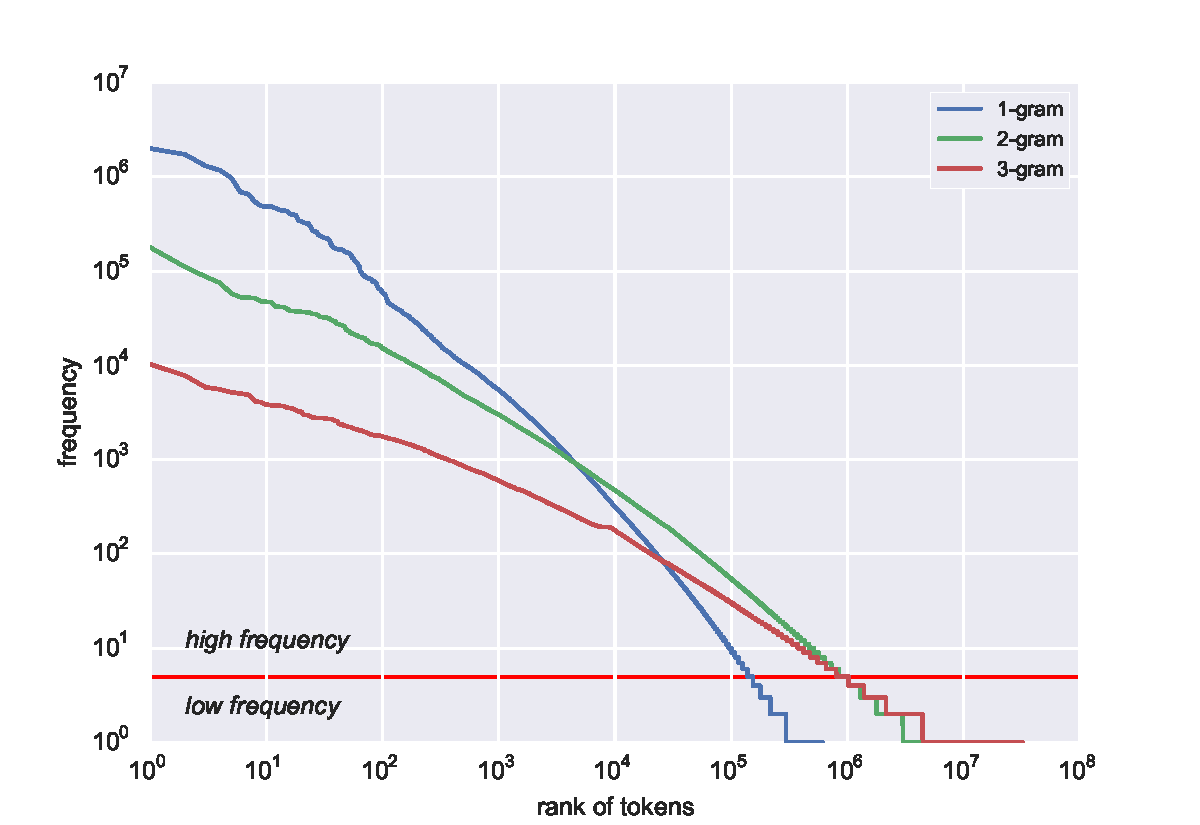
\includegraphics[width=0.8\textwidth]{fig/freqdist}
    \caption{Occurrence Frequency of terms in the corpus for uni-, bi- and trigram in descend ranking. The corresponding preprocessing is \iSE{} and the data source is \icontent{}.}
    \label{fig:freqdist}
\end{figure}

There are two main metrics to portray a vocabulary. The first metric is the size, which impacts the complexity of computing in next phases of discovering related articles. The second one is the scale of long tail of the vocabulary. According to the Zipf's law, the occurrence frequency is distributed extremely unevenly or that is to say that the most terms occur rarely in use and hence it is almost incapable to determine the semantic relevance of these terms by statistical methods. In ideal case, a vocabulary with smaller size and fewer not common used terms has the better quality with both of operational complexity and semantic completeness. Figure \ref{fig:freqdist}, which depicts a representative sample the distribution of the occurrence frequency, indicates that only a small quantity of tokens occur repetitively in the corpus (25\% for unigram, 10\% for bigram and 3\% for trigram). Taking into account efficiency, the tokens which appear less than $5$ times can be removed from the vocabulary. We denote the original vocabularies as \ifull{} vocabularies and the reduced vocabularies as \icommon{} vocabularies. 

\begin{figure}[!htb]
    \centering
    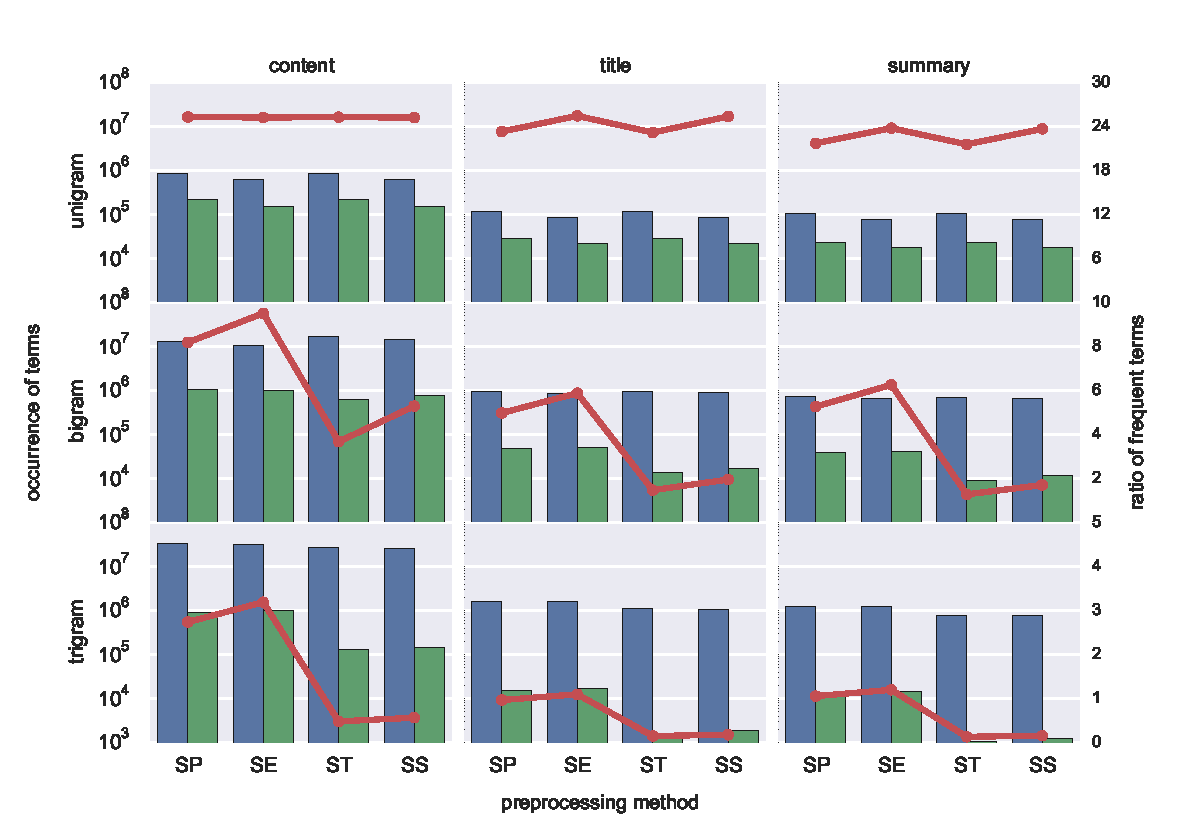
\includegraphics[width=\textwidth]{fig/vocab_size}
    \caption{Comparison the vocabulary size of different preprocessing methods for given data sources with n-gram models. Each column refers to a kind of data source, which is \icontent{}, \ititle{} and \isummary{} respectively while each row refers to a n-gram model: uni-, bi-, and trigram. \textit{Full} vocabularies are illustrated as blue bars and \icommon{} vocabularies as green bars. The red line shows the ratio of the size of \icommon{} vocabularies to the corresponding \ifull{} vocabularies. }
    \label{fig:vocab_size}
\end{figure}


We consider the size of \ifull{} vocabularies and the proportion of frequent tokens as the metrics to evaluate the vocabulary quality. Figure \ref{fig:vocab_size} shows the comparison between the size of \ifull{} and \icommon{} vocabularies which are generated by the preprocessing methods including \iSP{}, \iSE{}, \iST{} and \iSS{} in the different n-gram models ($n=1, 2, 3$) of the three kinds of data source containing \icontent{}, \ititle{} and \isummary{}. In the unigram model, \iSS{} always generates the both smallest vocabularies with the largest proportion of frequent terms. In bi- and trigram, the vocabularies generated by \iSE{} has the largest proportion of frequent terms and the size is slightly different with the vocabularies generated by other methods. In conclusion, the preprocessing method \iSS{} is applied in unigram and \iSE{} is applied in both of bigram and trigram. 


\subsection{Effectiveness of STS Models}
\label{sec:5.2}

As described in section \ref{sec:3.3}, the effectiveness metrics include \textit{precision@k@h} to evaluate the relatedness of the articles of top ranking and \textit{nDCG} to evaluate the overall results. First, the results for each data source with n-gram are given and the best STS models is selected respectively. We give a reasonable assumption that an article is related to the articles which are not farther than $3$ hops. In order to analyze the effectiveness, the assumption is relaxed or that is to say, that the effectiveness is evaluated in the cases of $1$-hop, $3$-hops, $5$-hops and $10$-hops. In the end of the section, the divergence between different categories is discussed and which categories the framework is more suitable for are concluded.  

\subsubsection{Parameter Selection for Topic Models}

Topic models, such as LSI and LDA, represent documents as vectors in topic space. The dimension of the topic space, as well as the number of topics is pre-defined. Hence, it is necessary to determine the optimal number of topics before building and evaluating models. Figure \ref{fig:precision_topics} shows the change in precision and operational time of LSI with increasing the number of topics from $50$ to $1000$. The precision keeps increasing but the growth becomes weaker and weaker, when the number of topics becomes larger. On the other side, the time cost of both of building and predicting increases with a relative stable growth speed. We selects $500$ as the final value of this hyperparameter, because the precision increases quiet insignificantly with more than $500$ topics and we expect that the building time is limited to less than one hour and the predicting time is limited to less than one second. 

\begin{figure}[!htb]
    \centering
    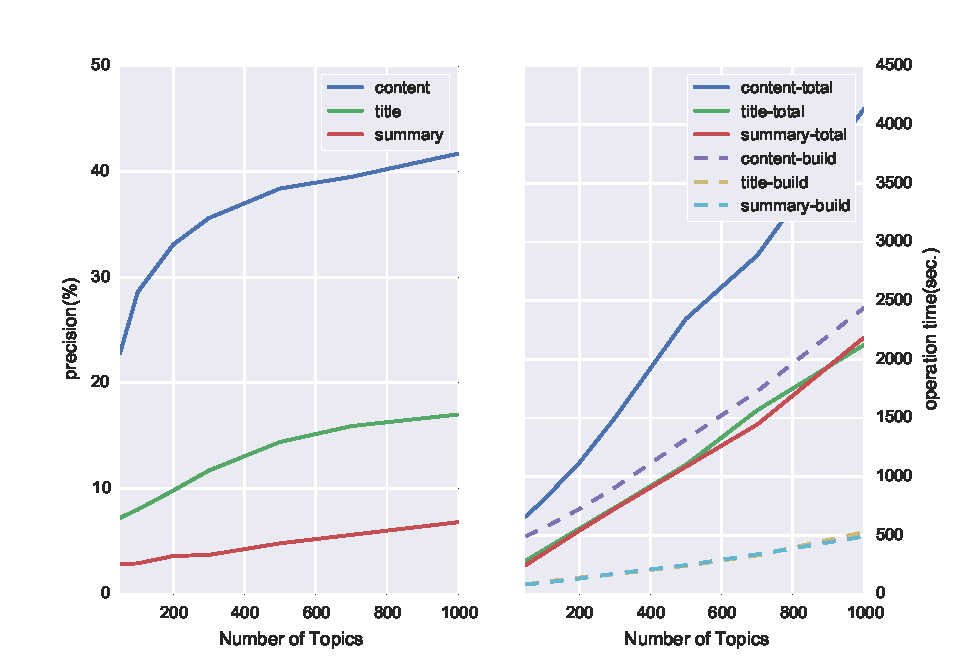
\includegraphics[width=\textwidth]{fig/precision_topics}
    \caption{Precision@2@3 and the time cost of LSI with the different value of the number of topics. Models are built with the historical corpus of $73908$ articles and predict related articles for $2000$ randomly selected articles. The dash line indicates the building time and the solid line indicates the total time including building and predicting. }
    \label{fig:precision_topics}
\end{figure}


\subsubsection{Model Selection}

The five STS models are applied for the nine separated semantic data ( (\icontent{}, \ititle{}, \isummary{}) $\times$ (unigram, bigram, trigram)). We apply \textit{precision@2@3} and \textit{nDCG} for evaluating the effectiveness of the models. 

Figure \ref{fig:precision_2_3} compares the precision of the STS models in the different data. In general, the models perform in \icontent{} better than in \ititle{} and much better than in \isummary{}. Second, the precision in unigram is better than in bigram and the precision in trigram is the worst. To be specific, \textit{tfidf} preforms the highest precision for all data sources in unigram and for \icontent{} and \ititle{} in bigram. In the meanwhile, \textit{Jaccard} is stronger than the other models for \isummary{} in bigram and all data sources in trigram. \textit{LDA} is the weakest model all the time in the experiment and it is skipped in bigram and trigram to avoid unnecessary costs. The precision of \textit{BoW} is slightly ($10\% \sim 30\%$) lower than the best model and, however, it is $30\% \sim 60\%$ lower than the best model in bigram and trigram. 


\begin{figure}[!htb]
    \centering
    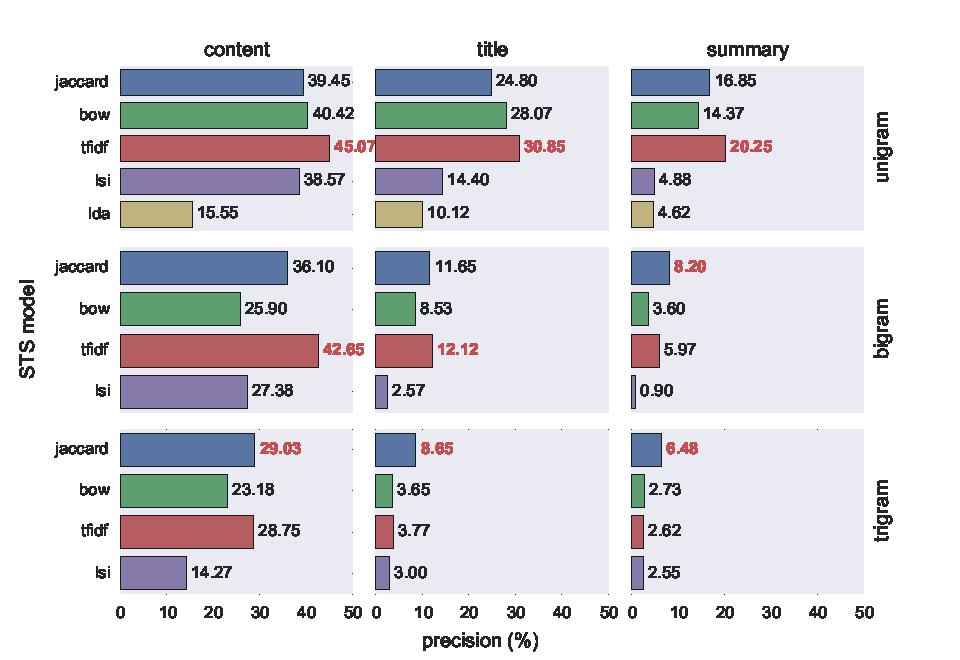
\includegraphics[width=\textwidth]{fig/precision_2_3}
    \caption{comparison the precision of \textit{jaccard}, \textit{BoW}, \textit{tfidf}, \textit{LSI} and \textit{LDA} for all data sources  with n-gram models. }
    \label{fig:precision_2_3}
\end{figure}

Figure \ref{fig:ndcg} illustrates the \textit{nDCG}, which is applied as the supplementary evaluation method. The order of models by \textit{nDCG} is similar to the results of \textit{precision} in general. All STS models are capable to discover related articles, because the measure \textit{nDCG} of every model is better than the baseline, which is computed for the random order of candidates. Moreover, LSI performs better in the metric \textit{nDCG} than in the metric \textit{precision} for the data source \icontent{}. To be specific, LSI is almost always at the second position after tfidf in \textit{nDCG}, whereas LSI is at the third or the last position in \textit{precision}. Accordingly, LSI computes the more precise relatedness of the overall corpus than jaccard and BoW, while LSI is not able to determine precisely which articles have the highest relatedness. 


\begin{figure}[!htb]
    \centering
    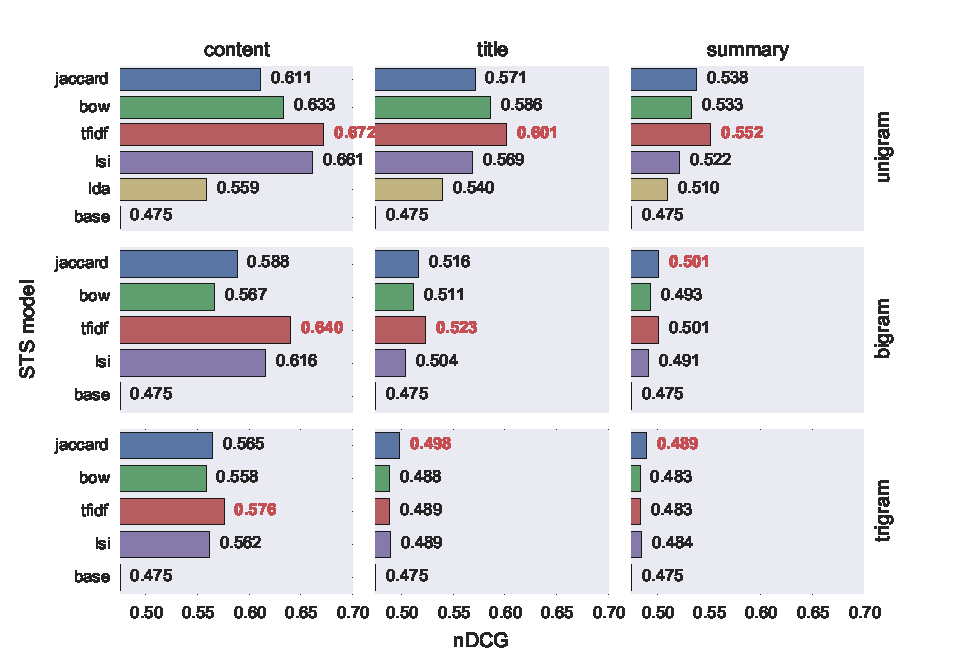
\includegraphics[width=\textwidth]{fig/ndcg}
    \caption{}
    \label{fig:ndcg}
\end{figure}


Combining the results of two evaluation methods, we conclude as follows.

1. Relatedness generated from data source \ititle{} or \isummary{} is worse than from \icontent{}, because \ititle{} and \isummary{} are short documents and then contain incomplete information. 

2. In n-gram, the vocabulary becomes larger and the relevance between phrases become weaker along with a greater $n$. On the other hand, a higher $n$ leads to the more serious loss of semantic information with removing the low frequency terms from the vocabulary. A typical example is that $77\%$ information/phrases are dropped through reducing vocabulary for \icontent{} in trigram. 

3. Tfidf is in the dominant position for uni-/bigram and long documents and jaccard is more suitable in trigram and short documents. Unexpected, LDA works with unsatisfactory effectiveness. 


\subsubsection{Coverage of Related Articles Prediction}

\begin{table}[]
\centering
\resizebox{\textwidth}{!}{%
\begin{tabular}{lrr|rr|rr|rr|rr|rr|rr|rr|rr}
 & \multicolumn{6}{c|}{\textbf{Content}} & \multicolumn{6}{c|}{\textbf{Title}} & \multicolumn{6}{c}{\textbf{Summary}} \\
 & \multicolumn{2}{c|}{\textbf{1-tfidf}} & \multicolumn{2}{c|}{\textbf{2-tfidf}} & \multicolumn{2}{c|}{\textbf{3-jaccard}} & \multicolumn{2}{c|}{\textbf{1-tfidf}} & \multicolumn{2}{c|}{\textbf{2-tfidf}} & \multicolumn{2}{c|}{\textbf{3-jaccard}} & \multicolumn{2}{c|}{\textbf{1-tfidf}} & \multicolumn{2}{c|}{\textbf{2-jaccard}} & \multicolumn{2}{c}{\textbf{3-jaccard}} \\
 & \multicolumn{1}{c}{\textbf{r}} & \multicolumn{1}{c|}{\textbf{diff}} & \multicolumn{1}{c}{\textbf{r}} & \multicolumn{1}{c|}{\textbf{diff}} & \multicolumn{1}{c}{\textbf{r}} & \multicolumn{1}{c|}{\textbf{diff}} & \multicolumn{1}{c}{\textbf{r}} & \multicolumn{1}{c|}{\textbf{diff}} & \multicolumn{1}{c}{\textbf{r}} & \multicolumn{1}{c|}{\textbf{diff}} & \multicolumn{1}{c}{\textbf{r}} & \multicolumn{1}{c|}{\textbf{diff}} & \multicolumn{1}{c}{\textbf{r}} & \multicolumn{1}{c|}{\textbf{diff}} & \multicolumn{1}{c}{\textbf{r}} & \multicolumn{1}{c|}{\textbf{diff}} & \multicolumn{1}{c}{\textbf{r}} & \multicolumn{1}{c}{\textbf{diff}} \\ \hline
\textbf{Average} & \multicolumn{2}{c|}{45.07} & \multicolumn{2}{c|}{42.65} & \multicolumn{2}{c|}{29.03} & \multicolumn{2}{c|}{30.85} & \multicolumn{2}{c|}{12.12} & \multicolumn{2}{c|}{8.65} & \multicolumn{2}{c|}{20.25} & \multicolumn{2}{c|}{8.20} & \multicolumn{2}{c}{6.48} \\ \hline
\textbf{\textcolor{blue}{Gesellschaft}} & 3 & $+~~8.75$ & 4 & $+~~6.89$ & 2 & $+17.38$ & 3 & $+15.20$ & 4 & $+13.20$ & 2 & $+53.01$ & 2 & $+14.98$ & 2 & $+28.53$ & 2 & $+43.84$ \\
\textbf{\textcolor{blue}{Politik}} & 4 & $+~~8.24$ & 1 & $+14.57$ & 1 & $+41.88$ & 4 & $+~~6.97$ & 6 & $+~~5.00$ & 5 & $+~~6.89$ & 1 & $+16.26$ & 3 & $+16.23$ & 3 & $+10.94$ \\
\textbf{Digital} & 1 & $+15.83$ & 2 & $+~~9.97$ & 7 & $-34.45$ & 1 & $+24.78$ & 5 & $+13.13$ & 7 & $-23.27$ & 3 & $+~~9.25$ & 6 & $-19.06$ & 8 & $-31.66$ \\
\textbf{Kultur} & 6 & $-~~5.28$ & 6 & $-~~9.53$ & 9 & $-52.02$ & 6 & $-~~3.05$ & 1 & $+44.99$ & 4 & $+~~8.22$ & 4 & $+~~3.73$ & 4 & $+14.16$ & 5 & $+~~5.78$ \\
\textbf{Lebensart} & 10 & $-34.97$ & 10 & $-35.32$ & 6 & $-28.72$ & 9 & $-27.35$ & 2 & $+42.20$ & 1 & $+59.46$ & 9 & $-31.89$ & 1 & $+47.18$ & 1 & $+59.77$ \\
\textbf{Sport} & 7 & $-~~7.26$ & 5 & $-~~8.71$ & 5 & $-18.10$ & 7 & $-16.31$ & 3 & $+35.20$ & 8 & $-24.19$ & 5 & $-~~8.93$ & 5 & $-~~5.04$ & 6 & $-~~5.06$ \\
\textbf{Wissen} & 2 & $+13.10$ & 3 & $+8.04$ & 4 & $-17.81$ & 2 & $+15.46$ & 9 & $-38.01$ & 9 & $-24.44$ & 7 & $-14.47$ & 9 & $-32.25$ & 10 & $-44.48$ \\
\textbf{Karriere} & 5 & $+~~6.58$ & 7 & $-12.65$ & 8 & $-42.58$ & 5 & $-~~1.48$ & 10 & $-43.40$ & 6 & $-20.66$ & 6 & $-12.85$ & 8 & $-28.26$ & 4 & $+~~5.99$ \\
\textbf{\textcolor{red}{Wirtschaft}} & 8 & $-14.73$ & 8 & $-17.52$ & 3 & $-13.03$ & 8 & $-19.23$ & 8 & $-36.87$ & 10 & $-26.57$ & 8 & $-15.55$ & 7 & $-20.55$ & 7 & $-11.96$ \\
\textbf{\textcolor{red}{Reisen}} & 9 & $-30.22$ & 9 & $-31.93$ & 10 & $-52.77$ & 10 & $-34.65$ & 7 & $-20.19$ & 3 & $+11.88$ & 10 & $-64.16$ & 10 & $-50.83$ & 9 & $-37.73$ \\
\textbf{\textcolor{red}{Studium}} & 11 & $-61.03$ & 11 & $-49.30$ & 11 & $-67.41$ & 11 & $-43.05$ & 11 & $-66.56$ & 11 & $-37.51$ & 11 & $-73.31$ & 11 & $-83.52$ & 11 & $-79.13$ \\ \hline
\end{tabular}%
}
\caption{My caption}
\label{my-label}
\end{table}

\subsubsection{Divergence between Categories}

以content-unigram为例,不同category有比较大的性能差异,XX最好,YY最差,相差ZZ\% 
在实际应用中,对于表现较弱的category,可以增加预测数量并加以人工筛查,以提高可用性。

\subsection{Efficiency of STS Models}
\label{sec:5.3}

1. building time

2. predicting time

\subsection{Results of Incremental Updating}
\label{sec:5.4}

\subsubsection{Effectiveness}

\subsubsection{Efficiency}

\subsection{Error Analysis}
\label{sec:5.5}

\subsection{Conclusion}
\label{sec:5.6}
